\documentclass[twoside]{article}
\setlength{\oddsidemargin}{0.25 in}
\setlength{\evensidemargin}{-0.25 in}
\setlength{\topmargin}{-0.6 in}
\setlength{\textwidth}{6.5 in}
\setlength{\textheight}{8.5 in}
\setlength{\headsep}{0.75 in}
\setlength{\parindent}{0 in}
\setlength{\parskip}{0.1 in}

\usepackage{graphicx}
\usepackage{url}
\usepackage{multicol}
\usepackage{listings}

%
% The following commands sets up the lecnum (lecture number)
% counter and make various numbering schemes work relative
% to the lecture number.
%
\newcounter{lecnum}
\renewcommand{\thepage}{\thelecnum-\arabic{page}}
\renewcommand{\thesection}{\thelecnum.\arabic{section}}
\renewcommand{\theequation}{\thelecnum.\arabic{equation}}
\renewcommand{\thefigure}{\thelecnum.\arabic{figure}}
\renewcommand{\thetable}{\thelecnum.\arabic{table}}
\newcommand{\dnl}{\mbox{}\par}

%
% The following macro is used to generate the header.
%
\newcommand{\lecture}[4]{
  \pagestyle{myheadings}
  \thispagestyle{plain}
  \newpage
  \setcounter{lecnum}{#1}
  \setcounter{page}{1}
  \noindent
  \begin{center}
  \framebox{
     \vbox{\vspace{2mm}
   \hbox to 6.28in { {\bf CMPSCI~630~~~Systems
                       \hfill Fall 2014} }
      \vspace{4mm}
      \hbox to 6.28in { {\Large \hfill Lecture #1  \hfill} }
%       \hbox to 6.28in { {\Large \hfill Lecture #1: #2  \hfill} }
      \vspace{2mm}
      \hbox to 6.28in { {\it Lecturer: #3 \hfill Scribe: #4} }
     \vspace{2mm}}
  }
  \end{center}
  \markboth{Lecture #1: #2}{Lecture #1: #2}
  \vspace*{4mm}
}

%
% Convention for citations is authors' initials followed by the year.
% For example, to cite a paper by Leighton and Maggs you would type
% \cite{LM89}, and to cite a paper by Strassen you would type \cite{S69}.
% (To avoid bibliography problems, for now we redefine the \cite command.)
%
\renewcommand{\cite}[1]{[#1]}

% \input{epsf}

%Use this command for a figure; it puts a figure in wherever you want it.
%usage: \fig{NUMBER}{FIGURE-SIZE}{CAPTION}{FILENAME}
\newcommand{\fig}[4]{
           \vspace{0.2 in}
           \setlength{\epsfxsize}{#2}
           \centerline{\epsfbox{#4}}
           \begin{center}
           Figure \thelecnum.#1:~#3
           \end{center}
   }

% Use these for theorems, lemmas, proofs, etc.
\newtheorem{theorem}{Theorem}[lecnum]
\newtheorem{lemma}[theorem]{Lemma}
\newtheorem{proposition}[theorem]{Proposition}
\newtheorem{claim}[theorem]{Claim}
\newtheorem{corollary}[theorem]{Corollary}
\newtheorem{definition}[theorem]{Definition}
\newenvironment{proof}{{\bf Proof:}}{\hfill\rule{2mm}{2mm}}

% Some useful equation alignment commands, borrowed from TeX
\makeatletter
\def\eqalign#1{\,\vcenter{\openup\jot\m@th
 \ialign{\strut\hfil$\displaystyle{##}$&$\displaystyle{{}##}$\hfil
     \crcr#1\crcr}}\,}
\def\eqalignno#1{\displ@y \tabskip\@centering
 \halign to\displaywidth{\hfil$\displaystyle{##}$\tabskip\z@skip
   &$\displaystyle{{}##}$\hfil\tabskip\@centering
   &\llap{$##$}\tabskip\z@skip\crcr
   #1\crcr}}
\def\leqalignno#1{\displ@y \tabskip\@centering
 \halign to\displaywidth{\hfil$\displaystyle{##}$\tabskip\z@skip
   &$\displaystyle{{}##}$\hfil\tabskip\@centering
   &\kern-\displaywidth\rlap{$##$}\tabskip\displaywidth\crcr
   #1\crcr}}
\makeatother

% **** IF YOU WANT TO DEFINE ADDITIONAL MACROS FOR YOURSELF, PUT THEM HERE:



% Some general latex examples and examples making use of the
% macros follow.

\begin{document}

%FILL IN THE RIGHT INFO.
%\lecture{**LECTURE-NUMBER**}{**DATE**}{**LECTURER**}{**SCRIBE**}
\lecture{3}{September 11}{Emery Berger}{Puja Mishra,Luis Almazan}

\section*{GitHub}
%\section{GitHub}

In the beginning of the class we saw a small introduction to GitHub and some commands.
\begin{itemize}
	\item \% git clone hhtps://(route) or ssht://(route)
	\item add (filename)
	\item commit -m "....."
	\item push
	\item pull
\end{itemize}

The professor also mentioned about how git works. In which upon creating a repository the Master branch is created. And that at anypoint time we could create more branches to work on our advances and changes, so we could keep committing and pushing to that particular branch, and later merge the other branches with the Master branch which has the "official" or working version of the code. And that per every push we would be able to see the differences which affect each file and change we are pushing.


\begin{figure}[ht!]
\center
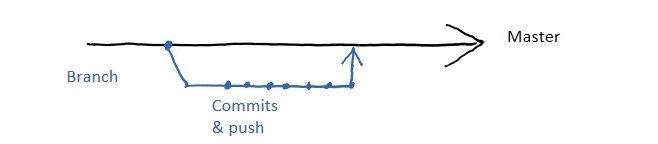
\includegraphics[width=150mm]{GitHub_Branches.jpg}
\caption{ GitHub Branches \label{ghBranches}}
\end{figure}

\section{Types of GC}

We have reviewed nine different types of Garbage Collectors. 
\begin{multicols}{3}
\begin{enumerate}
	\item Non-Moving
	\item Relocating (copying)
	\item Compacting
	\item Non-Compacting
	\item Stop-The-World
	\item Incremental
	\item Parallel
	\item Concurrent
	\item Generational
\end{enumerate}
\end{multicols}

The last 4 (Incremental, Parallel, Concurrent \& Generational) are not mutually exclusive. Meaning that one could have an Incremental-Parallel-Concurrent-Generational GC.

\subsection{Synchronous vs Asynchronous (Java vs C++)}

\begin{multicols}{2}

\subsubsection*{Synchronous(C++)}
Explicit Memory Management (Explicit declaration to reclaim object F)
\begin{lstlisting}[language=C++]
	f =  new Foo();
	.
	.
	.
	delete f;
\end{lstlisting}
\columnbreak

\subsubsection*{Asynchronous(Java)}
Constructor and destructor. There is a destructor but programmer can't know when GC will actually execute to reclaim the object.
\begin{lstlisting}[language=Java]
	Foo(){
	  .
	  .
	  .
	}

	~Foo(){
	  .
	  .
	  .
	}
\end{lstlisting}

\end{multicols}

\begin{enumerate}
	\item[*] The only way to use a mix of Asynchronous and Synchronous declarations is through \textbf{reference counting}.
	\item[*] System.GC type of instruction will be ignored by asynchronous GC's.
\end{enumerate}

\section{Leaky Abstraction}

We reviewed that an abstract approach is preferred in Systems. This approach is known as the Black-Box Abstraction  (Figure \ref{BB_Abstraction}). In this approach a set of black boxes would be implemented coupled by narrow interfaces. Ideally what happens in each box should be totally obscured and independent from the other. However there are several situations in which this boxes are not completely independent, or obscured, from one another, resulting in leaks. This phenomena is called \textbf{leaky abstraction}. The professor mentioned that due to performance advantages, some systems use designs which have leaky abstraction and in which the designer is aware of it. 

\newpage

\begin{figure}[ht!]
\centering
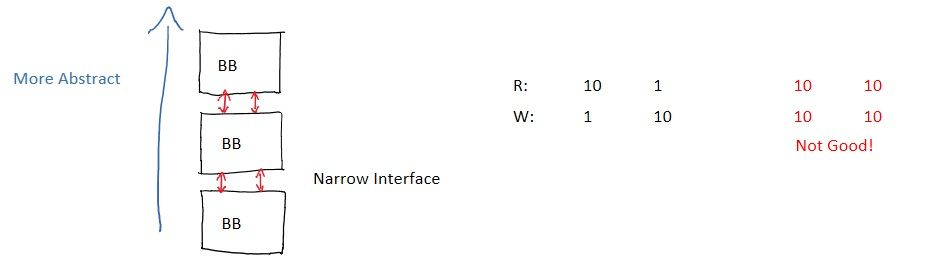
\includegraphics[width=150mm]{BB_Abstraction.jpg}
\caption{ Black-Box Abstraction \label{BB_Abstraction}}
\end{figure}

\section{Compacting}

\begin{figure}[ht!]
\center
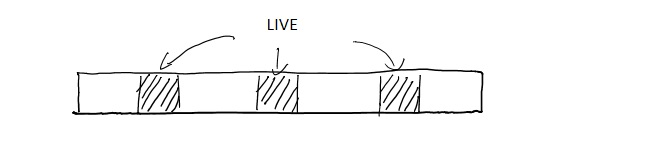
\includegraphics[width=150mm]{Compacting_Live.jpg}
\caption{ Live uncompacted ojects \label{compactingLive}}
\end{figure}

\subsection*{Objects}
\begin{itemize}
	\item \textbf{Reachable} \textit{(Missing definition)}
	\item \textbf{Live} Will be used in the future. (need to collect it conservatively)
	\item \textbf{Dead} Never to be used again.
\end{itemize}

\[ Live \subseteq Reachable \]

\[ Reachable \not\subset Live \]

Therefore GC should aim to use reachability not liveness.

\subsection{Static Analysis, Inter-procedural, compile time GC}
\begin{itemize}
	\item \textbf{Inter-procedural Analysis}.- using many procedures (not good!)

	\item \textbf{Intra-procedural Analysis} (good!)
	
	\item \textbf{Static Analysis} 
		
		\begin{lstlisting}[language=C++]
		a = ______
		b = ______
		.
		.
		.
		//Last use of A
		x = a;
		\end{lstlisting}

	\item \textbf{Conservative} (flow-insensitive)
	
	\item \textbf{Compile-Time GC} Insert deletes at compile time to the code (explicitly). However, it can't detect all, so far, and still is dependent on other run-time GC.
	
\end{itemize}

\subsection{Memory Leaks}

When you have more objects that are reachable but will never be used (live). An example where memory leak happens is in \textbf{Hash tables} (Figure\ref{hashTable}).

\begin{figure}[ht!]
\center
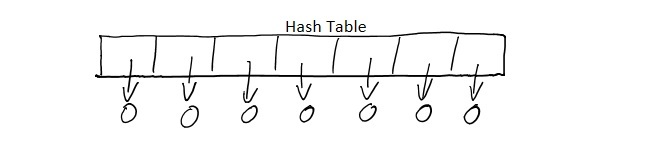
\includegraphics[width=150mm]{Hash_Table.jpg}
\caption{Hash Table \label{hashTable}}
\end{figure}

\begin{itemize}
	\item \textbf{Soft reference}.- special pointer that may never be pointing to something. Therefore it can be reclaimed.

	\item \textbf{Hard reference} 
\end{itemize}

\begin{figure}[ht!]
\center
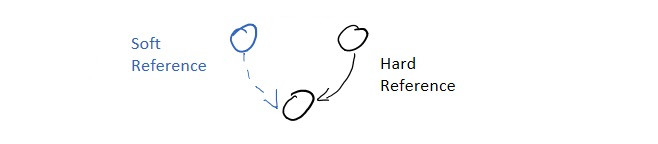
\includegraphics[width=150mm]{Soft_vs_Hard.jpg}
\caption{Soft vs Hard Referencing \label{softVsHard}}
\end{figure}

GC doesn't eliminate memory leaks but it eliminates premature reclamation of an object. 

\subsection{Java}

THIS NEEDS TO BE CHANGED (info comes from default template). DieHard is an allocator developed at UMass which provides (or at least
improves) soundness for erroneous programs.


\section{Mark - Sweep Compact}

Based on regular Mark Sweep but with the concept of compaction. Though it never copies. It just moves to rearrange the objects so objects that point to each other are in closer proximity when there are empty memory spaces in between.

\begin{figure}[ht!]
\center
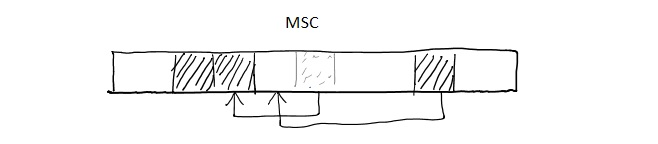
\includegraphics[width=150mm]{MSC.jpg}
\caption{ Mark Sweep Compact \label{markSweepCompact}}
\end{figure}

\section{Semi-space}

The memory is divided into two semispaces and memory is  allocated from the first semispace ("from") and the pointer is returned back to the object. After the end of the first semispace is reached all the memory which is still in use is copied to the next space ("to") leaving a forwarding pointer behind. Hence all the objects are copied and compacted everytime. And when the "to" space is full then the roles are switched and the "to" becomes "from" and vice-versa.

\begin{figure}[ht!]
\center
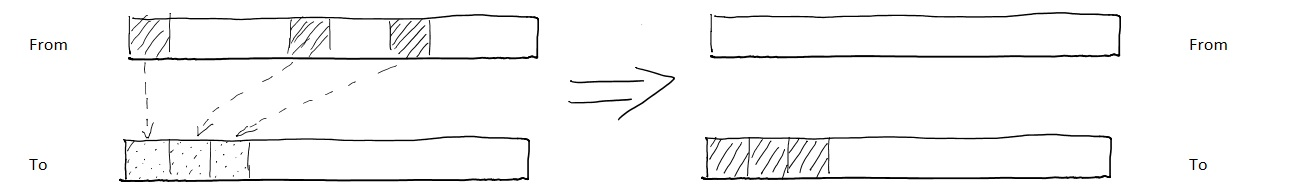
\includegraphics[width=150mm]{Semi_Space.jpg}
\caption{ Semi-Space GC \label{semiSpace}}
\end{figure}

The advantage of this technique is compacting happens at a very frequent rate and thus there is no fragmentation(fast allocation). The disadvantage is that it keeps copying object all the time which is very expensive and produces performance issues.

\[
	Fragmentation = \frac{Maximum Memory Used}{Maximum Memory Required}
\]


\begin{center}
	\textbf{In Compacting} \[Fragmentation = 1\]
\end{center}

\begin{center}
	\textbf{In Mark Sweep} 
	\[
		Fragmentation = log(\frac{size of largest object}{size of smallest object})
	\]
\end{center} 



In Mark Sweep without compaction fragmentation can be a big problem.

\begin{figure}[ht!]
\center
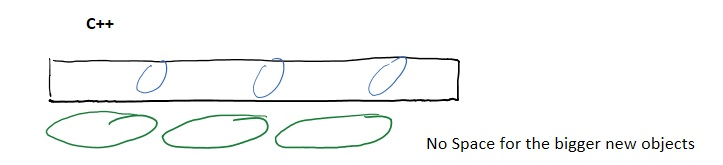
\includegraphics[width=150mm]{No_Compacting_Issues.jpg}
\caption{ Issues when No Compaction is Available \label{noCompactingIssues}}
\end{figure}

In theory, we saw an example of how fragmentation could be a real problem when you consider worst case scenario. The below examples were given:

\begin{multicols}{2}
\begin{center}
\[log(\frac{256B}{8B}) \approx 2.4 \]
\[log(\frac{1GB}{1B}) = 32 \] *(as seen in class)
\columnbreak
\[log(\frac{1GB}{1B}) = 9 \]
\[log(\frac{1TB}{1B}) = 12 \]*(from Google calculator)
\end{center}

\end{multicols}

In practice, \(fragmentation < 1.2\)  which is between \(20-30\%\).

\section{Types - Continued}

\subsection{Generational}

Generational GC is a hybrid of Mark-Sweep and Semi-Space.  It is based on a set of fast storage allocation spaces, which could be in Cache. This objects are considered \textbf{young}. It works similar as semi-space in which it would copy the live objects into a "to" space using compaction. There is a second space in memory where \textbf{old} objects live. If an old object points to a new object then this new object will become old (Figure \ref{generationalGC}).

It is based on the assumption that young objects will not live very long, and  therefore they will be collected soon. The space of memory where the young objects live is refered to as \textbf{The Nursery} or \textbf{Eden}. And the space where old objects live is called \textbf{remembered set}. The professor mentioned that there are more types of implementation of generational GC which may include different memory categories, Eg. \textbf{the immortals}.

\begin{figure}[ht!]
\center
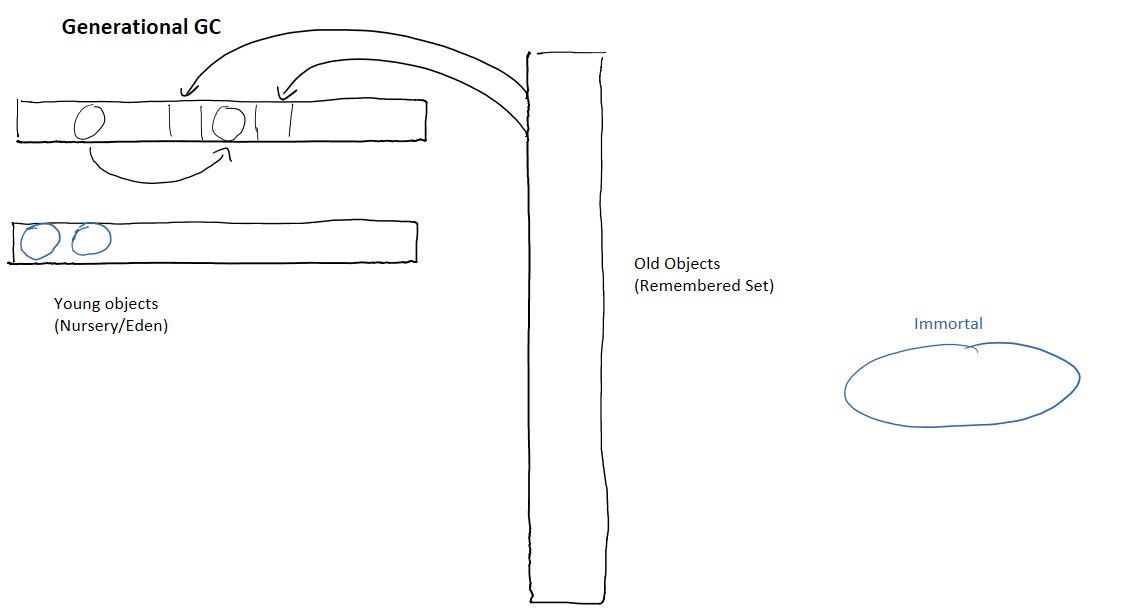
\includegraphics[width=150mm]{Generational.jpg}
\caption{ Generational GC \label{generationalGC}}
\end{figure}

\subsubsection*{High Performance Collection}
Languages that have a high performance collection use Generational GC since it is completely heuristic. It works as a buffer.

\begin{itemize}
	\item[*] \textbf{Pretenuring}.- Allocate new objects that seem to look old.
\end{itemize}

\subsection{Incremental}

Do some GC as the program is allocating memory (spread workout). 

\subsection{Parallel}

Launch multithread for as many cores as you have.


\subsection{Concurrent}

Happening at the same time as the program.

\begin{figure}[ht!]
\center
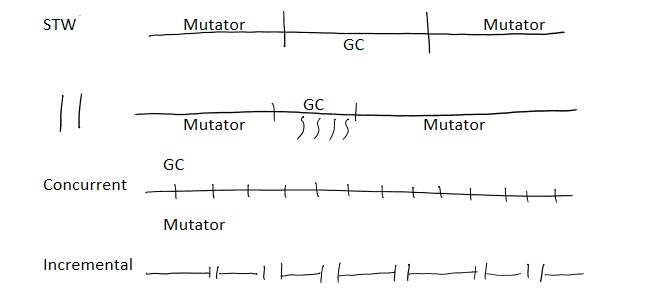
\includegraphics[width=150mm]{Types_GC.jpg}
\caption{ Mark Sweep Compact \label{typesGC}}
\end{figure}

\pagebreak

\section{Load Balancing}

The below diagram was briefly explained:

\begin{figure}[ht!]
\center
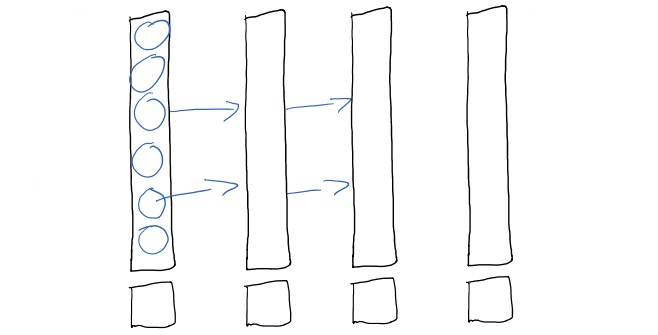
\includegraphics[width=150mm]{Load_Balancing.jpg}
\caption{ Load Balancing \label{loadBalancing}}
\end{figure}

\end{document}
